%----------------------------------------------------------------------------------------
%	8./ Calibration
%----------------------------------------------------------------------------------------
%\section{Calibration}
%\label{se:calibration}

We present the calibration of the absolute scale of the flux densities
for the NIKA2 instrument in this section using Uranus as the main
primary calibrator. Practically, at the stage of the FOV
reconstruction (see Sect.~\ref{se:geometry}), an absolute
coefficient factor per detectors is derived using a \bm\ scan of
Uranus. This step realizes also the inter-calibration of all the KID,
as the coefficient factors give the KID gains. Secondly, the flux
density absolute scale is further refined by monitoring the primary
calibrator all along the observation campaign to estimate an
absolute calibration correction.

We have evidenced a daily variation of the absolute calibration
coefficients as a function of the observation date, which is related
to temperature-induced variation of the beam size. If left uncorrected, this variation
induces a sizable increase of the calibration uncertainties. To
overcome this issue, we primarily flag the most impacted observation
dates and exclude the observations acquired during these periods. This
conservative approach constitutes the baseline calibration method,
which is further used for the performance assessment. For cross-check,
we also proposed an alternative method relying on a photometric
correction depending on the beam size. Both approaches require an
accurate monitoring of the beam size as a function of the observation
date.


First we describe the method for the absolute calibration in
Sect.~\ref{se:calibration_method}, then we present the
inter-calibration and the flat fields in
Sect.~\ref{se:flat_field}. The temperature-induced variation and the
beam size monitoring are then discussed in
Sect.~\ref{se:beam_variation}. Finally, the baseline calibration is
presented in Sect.~\ref{se:baseline_calibration} and the calibration
with a photometric correction in
Sect.~\ref{se:photometric_correction}.  



%---------------------------------------------------------------------
%	Method
%---------------------------------------------------------------------

\subsection{Absolute calibration procedure and photometric system}
\label{se:calibration_method}

We detail here the procedure for calibrating the absolute scale of
the flux density and the chosen photometric system.

\subsubsection{Photometric system}
\label{se:photometric_system}

The main primary calibrators of NIKA2 are the giant planets Uranus and
Neptune. The latter is used when the former is not visible in the most
stable observing conditions. The flux density expectations of the
primary calibrators are derived in Sect.~\ref{se:ref_flux_calibrator}. 

We parametrize the primary calibrator flux density
$S_{\rm{c}}(\nu) = S_{\rm{c}}(\nu_0)\, f(\nu/\nu_{0})$, where $f(\nu/\nu_{0})$
encloses the spectral dependence, 
as a function of a reference frequency $\nu_{0}$ that we choose
arbitrarily to be: $\nu_{0} = 150$~GHz for the 2mm array and
$\nu_{0}= 260$~GHz for both 1mm arrays. Projecting the raw data (in
units of the KID resonance frequency shift or $\rm Hz$) of a
calibrator, we model the raw map with a fixed-width Gaussian
\begin{equation}
  R_{\rm{c}}(\theta, \phi)  = \frac{A_{\rm{c}}}{2 \pi \sigma_{0}^{2}}
  e^{-\frac{\theta^{2}}{2\sigma_{0}^{2}}},
  \label{eq:gaussian_amplitude}
\end{equation}
where $\sigma_{0}$ is derived from the
reference FWHM, labelled FWHM$_{0}$, which are $12.5''$ for the 1mm
arrays and $18.5''$ for the 2mm array. These values have
been chosen sizably larger than the main beam values, as reported in
Sect.~\ref{se:beam}, to account for a fraction of the signal stemming from
the first error beam and first side lobes.
Both the reference frequency and FWHM, $\nu_0$ and FWHM$_{0}$, define our reference photometric system, as
summarized in Table~\ref{tab:definitions}.

\begin{table}[!htbp]
  \begin{center}
    \caption{NIKA2 reference frequencies and FWHM}
    \begin{tabular}{lcc}
      \hline\hline
      \noalign{\smallskip}
      & 1 mm & 2 mm \\
      \noalign{\smallskip}
      \hline
      \noalign{\smallskip}
      Reference frequency $\nu_{0}$ & 260 GHz & 150 GHz \\
      Reference FWHM  FWHM$_{0}$    & 12.5'' & 18.5'' \\
      \noalign{\smallskip}
      \hline
    \end{tabular}
  \end{center}
  \label{tab:definitions}
\end{table}

The absolute calibration coefficients are estimated as the ratio of
the flux density expectations at the reference frequency
$S_{\rm{c}}(\nu_0)$ and the amplitude estimate of the fixed-width reference
FWHM Gaussian $A_{\rm{c}}$. For any point-like source $\rm{s}$, the map
\begin{equation}
  M_{\rm{s}}(\theta, \phi) = \frac{S_{\rm{c}} (\nu_{0})}{A_{\rm{c}}}
  R_{\rm{s}}(\theta,\phi),
\end{equation}
where $R_{\rm{s}}(\theta,\phi)$ is the raw data projection, is calibrated in Jy/FWHM$_{0}$
beam. The flux density estimate for the source is then:
\begin{equation}
S(\nu_{0})  = \frac{S_{\rm{c}}(\nu_{0})}{A_{\rm{c}}} \, A_{\rm{s}},
\label{eq:pointsourcephot}
\end{equation}
where $A_{\rm{s}}$ is the amplitude estimate of a FWHM$_0$ Gaussian.

\subsubsection{Color correction}

The flux density estimate $S(\nu_{0})$ gives the
flux of the source at the reference frequency only if the source has
the same spectral index as the calibrator. In general, to retrieve the
flux of the source at the reference frequency, a color correction
$C_{\rm{s}}$ has to be applied
\begin{equation}
S_{\rm{s}}(\nu_{0}) = S(\nu_{0})  C_{\rm{s}}(\nu_{0}, \alpha_{\rm{s}}),
\end{equation}
which depends on the reference frequency $\nu_{0}$ and the source
spectral index $\alpha_{\rm{s}}$.
Neglecting the effect of the atmosphere on NIKA2 transmission, we compute the color correction
factor for target sources of spectral indices $\alpha_{\rm{s}}$ that are
different from Uranus using
\begin{equation}
  C_{\rm{s}}(\nu_{0}, \alpha_{\rm{s}}) = \frac{\int_{0}^{+\infty} (\nu/\nu_0)^{1.6} ~T({\nu}) d\nu}{ \int_{0}^{+\infty} (\nu
    /\nu_0)^{\alpha_S} ~ T({\nu}) d\nu}.
\end{equation}

Color correction factors for eight values of $\alpha_{\rm{s}}$, and in particular
for $\alpha_{\rm{s}}= 0.6$ which is the spectral index of MWC349, are
given in Table~\ref{tab:mod}. 

\begin{table*}[!h]
\caption{Color correction factor for a target source  $S \propto \nu ^{\alpha_{\rm{s}}}$}
\label{tab:mod}
\centering 
\begin{tabular}{l| c c c c c c c c}
\hline\hline
\noalign{\smallskip}
Array  & \multicolumn{8}{c}{$\alpha_{\rm{s}}$} \\
\noalign{\smallskip}
\hline
          &  -2 &  -1    &    0  & + 0.6 & +1  &  +2  & +3 & +4  \\
%            \noalign{\smallskip}
            \hline
%            \noalign{\smallskip}
          A1   & 0.876  &  0.916   &   0.951  & 0.969 &  0.981   &  1.005  &    1.024  &  1.037   \\
          A2   & 0.945  &  0.972   &   0.990  & 0.996 &  0.998   &  0.997  &    0.986  &  0.966      \\ 
          A3   & 0.907  &  0.940   &   0.967  & 0.980 &  0.987   &  1.001  &    1.009  &  1.011     \\
            \noalign{\smallskip}
            \hline
\multicolumn{8}{c}{Note : Uranus/Moreno model used for Uranus in this
  Table.}
\end{tabular}
\end{table*}


\subsubsection{Diffuse source}
\label{se:extended_source_calib}
For aperture photometry or for extended sources, the map calibrated in
Jy/FWHM$_{0}$ must be converted in a map in Jy/sr, that is corrected
with the reference beam efficiency, defined as the ratio of the solid
angle enclosed in the reference fixed-width Gaussian beam and the
solid angle of the total beam. The total solid angle estimates are
presented in Sect.~\ref{se:beam_efficiency}. The reference beam efficiencies
are given in Table~\ref{tab:reference_beam_efficiency}.


\begin{table}[!thbp]
  \caption[]{Reference beam efficiencies for Array 1, Array 3, Array
    1\&3 and Array 2}
  \label{tab:reference_beam_efficiency}
  \centering    
  \begin{tabular}{lrrrr}
    \hline\hline
    \noalign{\smallskip}
    & A1 & A3  & A1\&3 & A2 \\
    \noalign{\smallskip}
    \hline
    \noalign{\smallskip}
    FWHM$_{0}$ [arcsec]          &  $12.5$   &  $12.5$  &   $12.5$  &   $18.5$  \\
    B.E$_{0}$\tablefootmark{a}\hspace{3mm}  [\% ] & $70 \pm 4$ & $72 \pm 4$ & $70 \pm 4$ & $85 \pm 3$ \\
    \hline
  \end{tabular}
  \tablefoot{ \\
    \tablefoottext{a}{Reference Beam Efficiency, estimated as the ratio between the reference FWHM beam power and the total beam power up to a radius of 180 arcsec} 
  }
\end{table}


\subsubsection{Practical calibration}
\label{se:practical_calib}
Practically, the absolute calibration consists in evaluating a flux
density rescaling factor using a series a OTF scans toward
Uranus or Neptune. This flux rescaling factor is an estimate of the
$S_{c}(\nu_{0})$-to-$A_{c}$ ratio of Eq.~\ref{eq:pointsourcephot}. The
calibrator flux density expectation $S_{c}(\nu_{0})$ is obtained as
discussed in Sect.~\ref{se:ref_flux_uranus_neptune}, whereas the measured
amplitude $A_c$ is estimated as the average amplitude of the $FWHM_0$
Gaussian fitted from a series of calibrator maps.

Before the flux density estimation, the calibrator raw data are i)
intercalibrated as decribed in Sect.~\ref{se:flat_field} and ii) corrected for the
atmospheric attenuation as described in Sect.~\ref{se:opacity}. To
refine the intercalibration between the two $1$-mm arrays after the
KID Hertz to Jy/beam conversion factor estimates, a flux rescaling
factor per array is calculated.

The primary calibrator observation scans are selected as discussed in
Sect.~\ref{se:data_selection}. In addition to the scan selection cuts,
we use a Gaussian beam size criterion. The FWHM estimated from the planet
observation map is required to be lower than $12.5''$ at $1\,\rm{mm}$ and lower
than $18''$ at $2\,\rm{mm}$. In further mitigating the flux scatter
due to beam broadening, we ensure better accuracy of the absolute
calibration.



%---------------------------------------------------------------------
%	INTERCALIBRATION
%---------------------------------------------------------------------
\subsection{Relative calibration \& flat fields}
\label{se:flat_field}
While absolute calibration of each KID also \emph{de facto} provides
relative calibration, the latter is interesting in itself to
characterize the instrument. We focus on this aspect in this
section.

The dispersion of the detector responsivity across the field of view (\aka\ flat
fields) has been characterized in several ways:

\noindent \emph{Main beam flat fields:} These are the FOV distributions
of the calibration coefficient of each KID, which correspond to the
PSF response to a point source in the far field of the
telescope. The calibration coefficients are estimated using a \bm\ scan
of a calibrator, as discussed in Sect.~\ref{se:photometric_system}. We
further clarify the computation of the calibration coefficient $G_k$
for the KID $k$ as:
\begin{equation}
  G_k = \frac{S_{th}(\nu_0)\, e^{-\tau/sin(\elev)}}{A_k}, 
\end{equation}
where $S_{th}(\nu_0)$ is the expected flux density of the source at
the reference frequency $\nu_0$, $\tau/sin(\elev)$ is the
line-of-sight opacity measured using the NIKA2 skydip-based method
(see Sect.~\ref{se:opacity}) and $A_k$ is the
amplitude of the reference FWHM$_0$ Gaussian, which is fitted in the
KID map using Eq.~\ref{eq:gaussian_amplitude}.

\noindent \emph{Forward beam flat fields:} These are the FOV
distributions of the relative response of
each KID to the near field atmospheric background. They are estimated
using the correlation factor of each detector TOI 
to a median common mode estimated off-source (see Sect.~\ref{se:toi_proc} for
more details on common modes).

Figure~\ref{fig:avg_mbff} %and \ref{fig:avg_fbff}
show the average main beam %and forward beam
flat field for the three arrays. These have been constructed by
combining the normalized flat fields of five \bms, which were
selected by thresholding the line-of-sight opacity measured in the
1\,mm band to $\tau/sin(\elev) \leq 0.85$. The distributions for the average flat
fields are shown in the bottom panel of Fig.~\ref{fig:avg_mbff}.% and \ref{fig:avg_fbff}.

We observe a sizable variation of the flat fields for A1 from the left-most side
to the right-most side of the FOV: this reveals a significant change of A1
detector responsivities depending on their position in the FOV. Namely, this
effect mainly impacts the South-West third of the array, which is
referred to as the "shadow-zone''. This variation of the
flat field translates into a broadening of the distribution. However, we verified that A1's
flat field dispersions are in line with the ones of A3 after the
detectors within the shadow-zone were flagged out using a
crescent-shaped mask. The masked flat field distributions are shown in
green in Fig.~\ref{fig:avg_mbff}, %and \ref{fig:avg_fbff}
whereas shadow-zone distributions are in red. The same FOV patterning
is also observed in the forward beam flat fields, which excludes a
main beam related issue. 

%In addition to the average flat fields, we further
%characterize the flat fields for individual \bms. Fig.~\ref{fig:stddev_ff}
%shows the dispersion of the flat fields for nine \bms\ using
%either the whole FOV or masking the shadow-zone. The dispersion estimates for
%this two cases are gathered in Table~\ref{tab:flatfield_res}.
%While the
%shadow zone is exluded, the A1 flat field dispersions are reduced by a
%factor of about two, and reached values close to that of the A3 flat
%field dispersions, while the latters are unchanged. 

%\begin{table}[!h]
%\begin{center}
%\begin{tabular}{|l|l|c|c|c|}
%\hline
% Dispersion ($\%$)    & KID selection  &  A1 & A3  & A2 \\
%\hline
%Main beam flat field  & all the FOV           & $34.4 \pm 3.4$    & $15.5 \pm 1.4$  &  $13.2 \pm 1.7$  \\
%                      & shadow-zone excluded  & $17.0 \pm 1.1$    & $14.2 \pm 1.2$  &  $12.8 \pm 1.3$\\
%\hline
%Forward beam flat field  & all the FOV           & $21.6 \pm 1.4$  & $10.1 \pm 1.7$  & $5.2 \pm 0.9$   \\
%                         & shadow zone excluded  & $12.2 \pm 1.6$  & $10.1 \pm 2.1$  & $4.9 \pm 1.2$ \\
%\hline
%\end{tabular}
%\caption[Flat field dispersions]{Average flat field dispersions in percent for
%  nine \bms\ over all the FOV and after masking out the shadow-zone}
%\label{tab:flatfield_res}
%\end{center}
%\end{table}

\begin{figure*}[!thbp] 
\begin{center}
  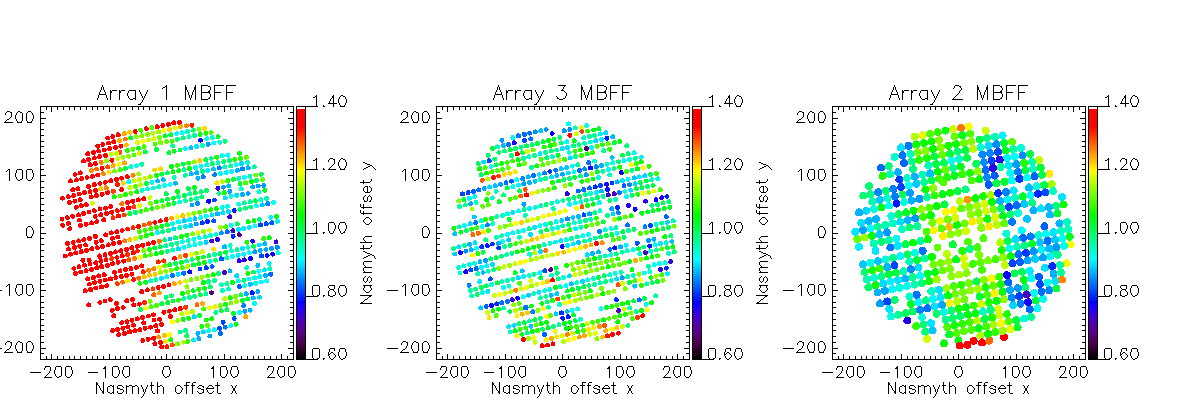
\includegraphics[width=0.95\textwidth]{Figures/Average_main_beam_flat_field_N2R9_10.png}
  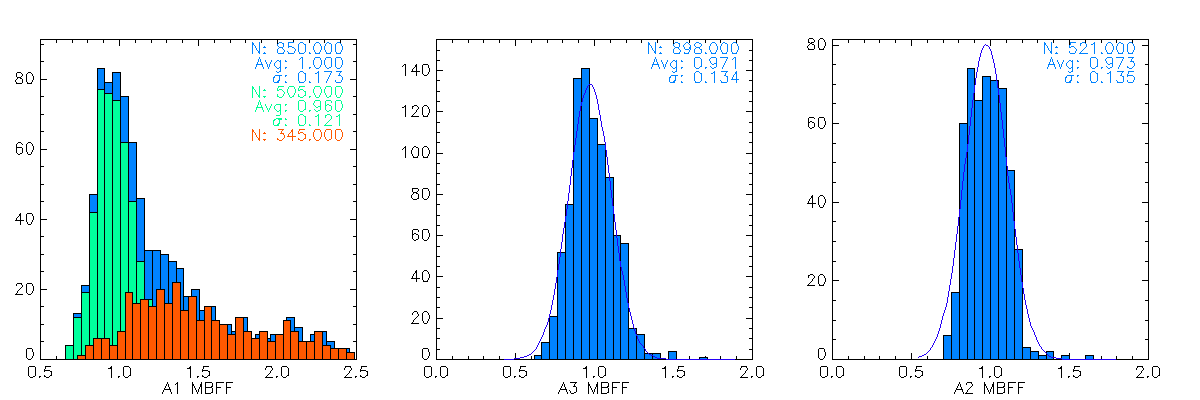
\includegraphics[width=0.8\textwidth]{Figures/Histo_average_main_beam_flat_field_N2R9_10.png}
\caption[Average main beam flat fields]{Average main beam flat fields
  obtained by combining the normalized flat fields of five
  \bm\ scans. The top row plots show the average flat fields of Array
  1, 3 and 2 in Nasmyth coordinates, and the bottom plots
  show the average flat field distributions using all KIDs (blue),
  using Array 1 KIDs that are positioned out of the shadow zone
  (green) and using Array 1 KIDs inside the shadow zone, which is
  defined in the text.}
 \label{fig:avg_mbff}
\end{center}
\end{figure*}

%\begin{figure*}[!thbp] 
%\begin{center}
%  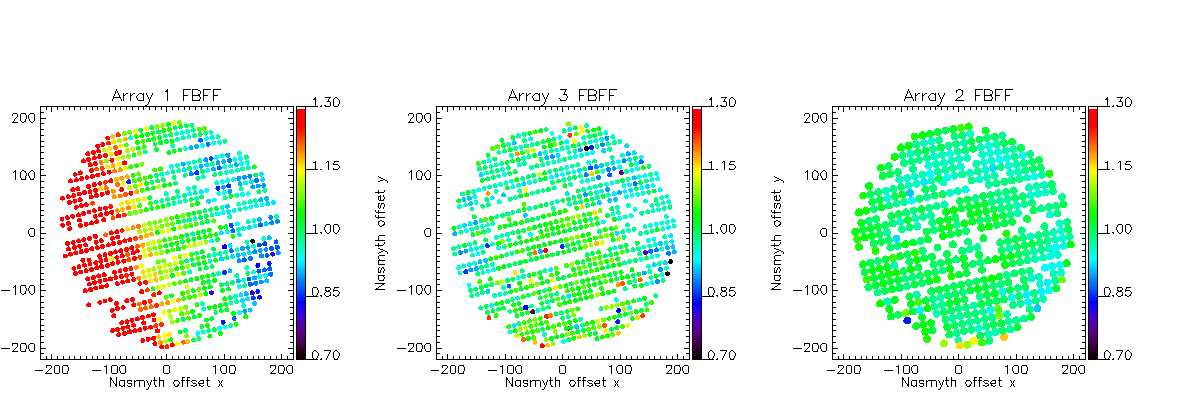
\includegraphics[width=0.95\textwidth]{Figures/Average_near_beam_flat_field_N2R9_10.png}
%  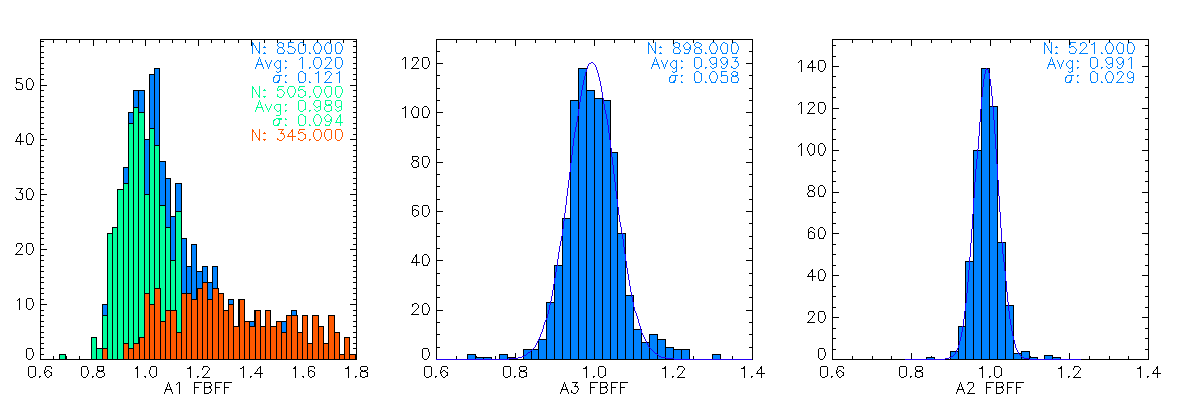
\includegraphics[width=0.8\textwidth]{Figures/Histo_average_near_beam_flat_field_N2R9_10.png}
%\caption[Average forward efficiency flat fields]{Average forward efficiency flat field for array 1, 3 and
%  2. Same legend as Fig.~\ref{fig:avg_mbff}}
% \label{fig:avg_fbff}
%\end{center}
%\end{figure*}

%\begin{figure}[ht] 
%\begin{center}
%  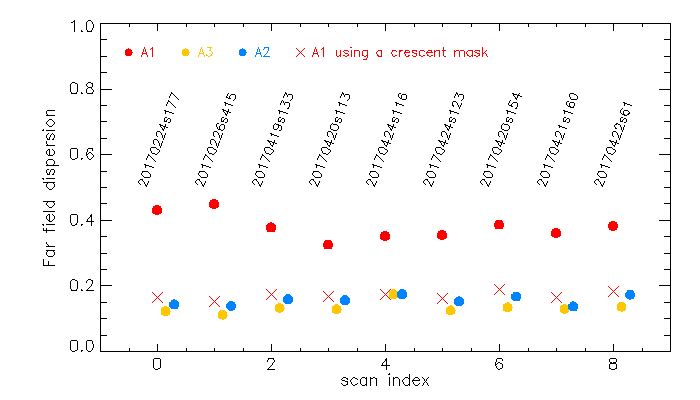
\includegraphics[width=0.6\textwidth]{Figures/FlatFields/Dispersion_main_beam_flat_field_N2R9_10_.png}
%  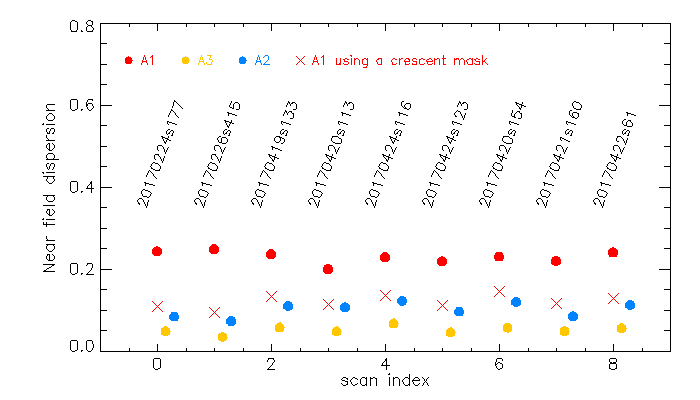
\includegraphics[width=0.6\textwidth]{Figures/FlatFields/Dispersion_forward_beam_flat_field_N2R9_10_.png}
%\caption[Dispersion of the flat field for nine \bms.]{The RMS
%  dispersion of the normalised main beam flat field (upper panel) and forward beam flat
%  field (lower panel) are shown using all valid KIDs of Array 1 (red circles),
%  Array 3 (orange circles) and Array 2 (blue circles), and using the KIDs
%  located outside the Array 1 "shadow zone'', which was discarded using a left
%  crescent-shaped mask (red crosses).}
% \label{fig:stddev_ff}
%\end{center}
%\end{figure}

The shadow zone effect is caused by an unexpected attenuation of
the transmission of the $1\,\rm{mm}$ polarisation that illuminates
A1 due to a characteristic of the dichroic which is out of
specifications.
This effect,
which implies a wrong placement of the transition zone of the dichroic
that depends on frequency, incidence angle and polarisation, is 
reproduced using optics simulation. This explanation has then been
verified using obervation at the technical campaign of September
2018. During this test campaign, a new \emph{hot-pressed} dichroic had
been installed in place of the current \emph{air-gap} dichroic.
Whereas the latter is made of a series of thin
micron-like membranes separated by calibrated rings and mounted on
a native ring in inox, the new hot-pressed dichroic consisted of a
rigid disk of plastic with a thickness of about $2\,\rm{mm}$ mounted on a
plastic ring. The shadow zone variations of the flat field for A1 were
not observed during the September 2018 campaign, while huge distortions
across the field of view of A2 were reported. The air-gap dichroic,
which is more immune to deformation than the hot-pressed one, has been
re-installed at the end of the September 2018 run. This test has
confirmed that the shadow zone effect was due to incoming radiation
absorption by the current air-gap dichroic.



%---------------------------------------------------------------------
%	TEMPERATURE-INDUCED VARIATION
%---------------------------------------------------------------------
\subsection{Temperature-induced variations}
\label{se:beam_variation}
We evidenced a daily variation of the flux density estimates,
which correlates with the beam size estimates.
This beam size broadening, which depends on the
scan observation date and mainly impacts late
afternoon observations, is reproducible from a campaign to another and 
is probably due to deformations of the main dish subject to the Sun
heating. This is a well-known effect, which also impacts EMIR and was
observed for the previous generation of instrument MAMBO. However,
compared to the period when MAMBO or NIKA were on activity, these
daily deformations have probably strengthen due to the ageing of the
main dish white coating. On short time scales, anomalous refraction
may also play a role~\citep{Altenhoff1987}. Based on observation
experience with EMIR, afternoon hours were often impaired with an
unstable atmosphere while rising moist air that
moves through the beam of the telescope causes the telescope beam
position to change within few seconds by several arcseconds.

The impact of this effect on the flux density estimates can be
mitigated, as we will explain in
Sects.~\ref{se:baseline_calibration}-\ref{se:photometric_correction},
provided the temperature-induced beam variations are accurately
monitored. Here, we describe the methods to monitor the beam size.   


\subsubsection{Beam monitoring using bright source scans}
\label{se:beam_monitoring_otf}

The time-dependent beam-size variations are primarily monitored using
all the available bright source scans acquired at the optimal focus
for each campaign. Bright sources are selected by thresholding the
flux density estimates above $1\,\rm{Jy}$ at both wavelengths.
The beam size is estimated by fitting a 2D Gaussian from the map and
taking the geometrical FWHM, defined as 
$\rm{FWHM}_{\rm{geom}} = (\rm{FWHM}_x \rm{FWHM}_y)^{1/2}$, where
$\rm{FWHM}_x$ and $\rm{FWHM}_y$ are the best-fitting values of FWHM
along the minor and major axis of the elliptical 2D Gaussian.
% see def of RESULT_FWHM in nk_grid2info.pro line 320
% + see def of params in nika_gauss2d.pro
For Uranus, the FWHM estimates are corrected for the beam broadening due
to the finite extension of the apparent disc, as in Sect.~\ref{se:mainbeam}. 

\begin{figure}[ht!]
  \begin{center}
    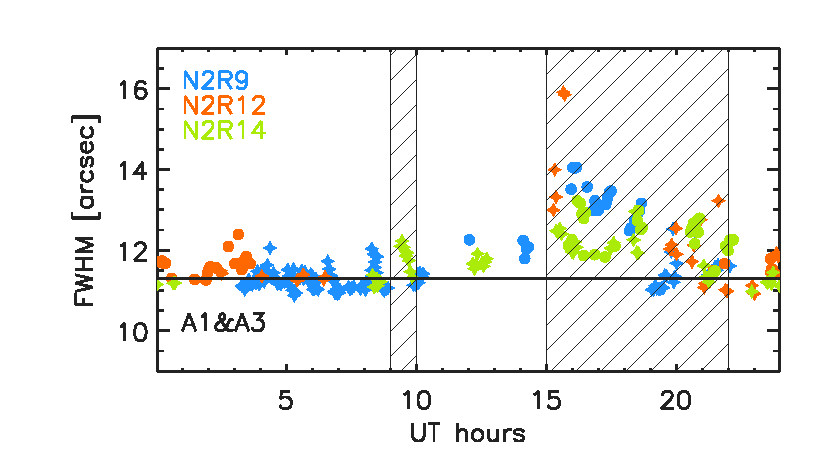
\includegraphics[clip=true, trim={0.9cm, 0.5cm, 0.5cm, 0.5cm}, width=0.4725\textwidth]{Figures/Beam_monitoring_with_otfs_vs_ut_1mm.pdf}
    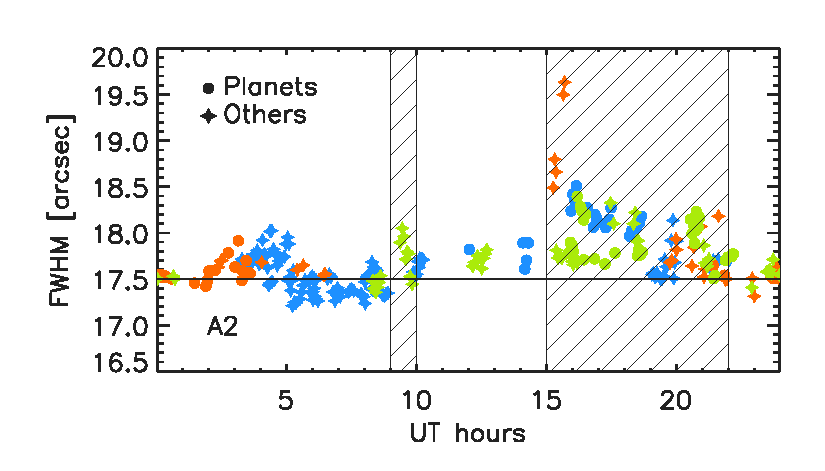
\includegraphics[clip=true, trim={0.5cm, 0.5cm, 0.5cm, 0.5cm}, width=0.4875\textwidth]{Figures/Beam_monitoring_with_otfs_vs_ut_a2.pdf}
    \caption[Beam size monitoring using OTF scans]{Beam size
      monitoring using OTF scans. FWHM at $1\,\rm{mm}$ (left panel)
      and $2\,\rm{mm}$ (right panel) as a function of the
      observation time in UT hours are shown using scans of giant
      planets (filled circles) and bright point-like sources above
      $1\,\rm{Jy}$ (filled stars) for N2R9 commissioning campaign and
      N2R12 and N2R14 science pools. The cross-hatched areas
      correspond to observing time period that are discarded using
      the baseline selection, as decribed in Sect.~\ref{se:data_selection}.} 
\label{fig:beam_monitoring_otf}
  \end{center}
\end{figure}

Figure~\ref{fig:beam_monitoring_otf} shows the geometrical FWHM as a
function of the observing time of the scans in UT hours for all OTF
scans of bright sources for the N2R9 commissioning campaign as well
as for the N2R12 and N2R14 science pools. For the three campaigns, we
observe the same evolution of the FWHM, which goes from a plateau at a
median value of $11.3''$ at $1\,\rm{mm}$ and $17.5''$ at $2\,\rm{mm}$
during the night, to a smooth rise that reaches a maximum of about $14''$
at $1\,\rm{mm}$ and $18.5''$ at $2\,\rm{mm}$ around 16:00 UT
hours. The beam broadening begins to become sizable around 15:00 UT
and one has to wait until around 22:00 UT for the beam sizes to lay
down on the stability plateau. The UT time ranges that are discarded
using the baseline scan selection (see
Sect.~\ref{se:data_selection}) are shown as cross-hatched areas in
Fig.~\ref{fig:beam_monitoring_otf}. They correspond to the afternoon
period between 15:00 and 22:00 UT hours, that is when the
telescope main dish is heated by daylight, as well as the
9:00-to-10:00 Sun rising period. The same beam size variations in time
using scans of giant planets (Uranus and Neptune) or other bright
sources (mainly quasars) are observed. However, FWHM from planets
observation tend to be slightly larger than FWHM from the observation
of other sources. This originates from larger 2D Gaussian fitted
values due to the error beams, which are measured with a
signal-to-noise as higher so as the source is bright. This small
effect is accounted for the beam-dependent calibration cross-check
discussed in Sect.~\ref{se:photometric_correction}.


\subsubsection{Beam monitoring using pointing}
\label{se:beam_monitoring_pointing}

For a finer sampling of the observation hours, we also consider using
the pointing scans for beam monitoring. As discussed in
Sect.~\ref{se:pointing}, the telescope pointing is
monitored on a hour basis during observation using pointing
scans. Furthermore, as they consist of two sub-scans in azimuth and
elevation of about 10 seconds of integration time each, pointing scans
can also be used to make a map of the pointing source. For each campaign,
we thus have on hand hundreds of maps of mostly point-like bright
sources. These can be also used to monitor the beam size, although we
expect less accuracy than using standard bright source scans due to the
shorter integration time and the fact that only the centermost KIDs in
the array see the source.  

%traitement pointing scans
For this purpose, pointing scans are reduced using
the data analysis pipeline described in
Sect.~\ref{se:dataproc} with the same parameters as for
standard OTF scans, and projected onto maps of $2''$ resolution.
As previously, an elliptical 2D Gaussian is then fitted from the map
and a geometrical FWHM is formed from the best-fitting FWHM along the
two ellipse radii. FWHM estimates on Uranus maps are corrected for an
offset due to the finite size of the apparent disc, as discussed in
Sect.~\ref{se:beam_monitoring_otf}. Pointing scans on other extended
sources, such as NGC7027, are discarded from the analysis.

% anomalous refraction
For each pointing, we also seek for atmospheric anomalous refraction. There are
enough KIDs per observation band to make an independent map using only
one subscan, i.e. 10 seconds of integration time.
For each of the four cross subscans, we thus estimate the position of the best
2D Gaussian that fits the map. We compute the deviation between each
subscan-derived position and the best-fit position using the entire
scan. An anomalous refraction event is detected when the deviation is
above $2.5''$ for at least one subscan. We find that the apparent beam
broadening during afternoons is due to anomalous refraction for
between one third and one half of the scans.%\footnote{See the study posted
%  in the commissioning internal wiki at
%  \url{http://www.iram.fr/wiki/nika2/index.php/Millimetric_anomalies_(weather,_antenna)_as_monitored_by_pointing_scans}}.
%} 

%In Fig.~\ref{fig:beam_monitoring_pointing}, we present the FWHM
%estimates using pointing scans as a function of the observing time in
%UT hours for three observation campaigns. We observe the same beam
%size evolution with UT hours as previously discussed in
%Sect.~\ref{se:beam_monitoring_otf}, that is a plateau during night-time
%and a smooth increase during day-time up to a maximum in the
%afternoon, which is followed by a smooth decrease down to the plateau
%a few hours after the sunset. Although the general trend is the same
%as the OTF-based FWHM variations, more dispersion is seen either using
%pointings toward giant planets or other bright sources.
%
%\begin{figure}[ht!]
%  \begin{center}
%    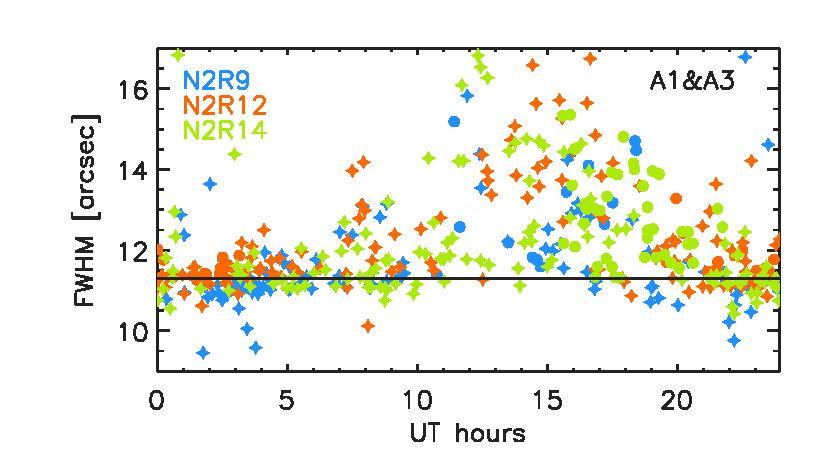
\includegraphics[clip=true, trim={0.9cm, 0.5cm, 0.5cm, 0.5cm}, width=0.4725\textwidth]{Figures/Beams/Beam_monitoring_with_pointings_vs_ut_1mm.pdf}
%    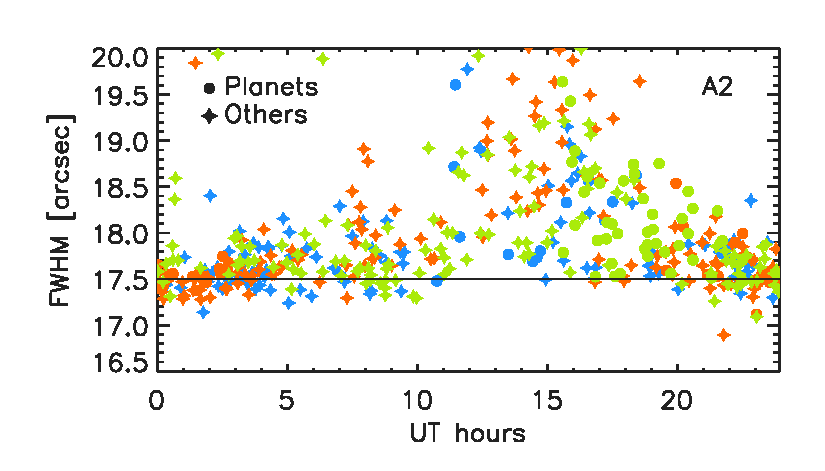
\includegraphics[clip=true, trim={0.5cm, 0.5cm, 0.5cm, 0.5cm}, width=0.4875\textwidth]{Figures/Beams/Beam_monitoring_with_pointings_vs_ut_a2.pdf}
%    \caption[Beam size monitoring using pointing scans]{Beam size
%      monitoring using pointing scans. Same legend as in
%      Fig.~\ref{fig:beam_monitoring_otf}.} 
%\label{fig:beam_monitoring_pointing}
%\end{center}
%\end{figure}
%
The pointing-based FWHM constitute a time-sampling of the FWHM during
the whole observation campaign. They can serve to estimate the beam
size of any observation scans, in particular
toward sources too faint for a direct FWHM fit to be made on the
projected map. To mitigate the dispersion, the time-stamped
pointing-based FWHM is filtered with a running median on a 70-minute
width time window. Then, the FWHM at the time of the considered scans is
interpolated from the smoothed pointing-based time-stamped FWHM.
%
\begin{figure}[ht!]
  \begin{center}
    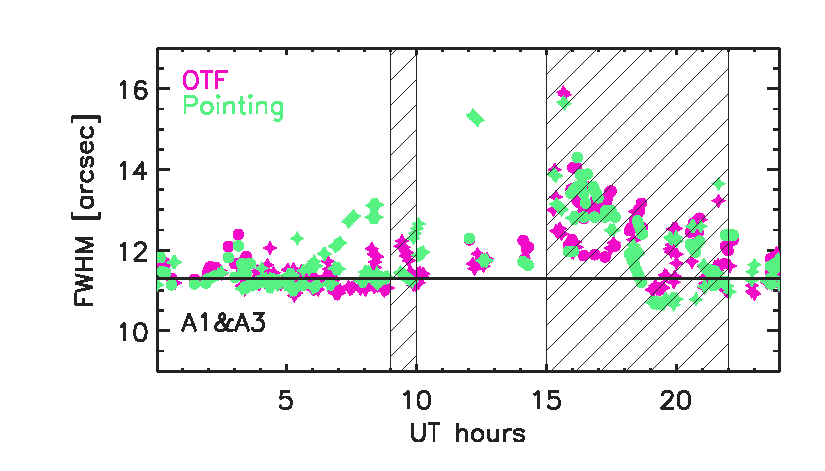
\includegraphics[clip=true, trim={0.9cm, 0.5cm, 0.5cm, 0.5cm}, width=0.4725\textwidth]{Figures/Beam_monitoring_with_otfs_vs_ut_compare_pointings_1mm.pdf}
    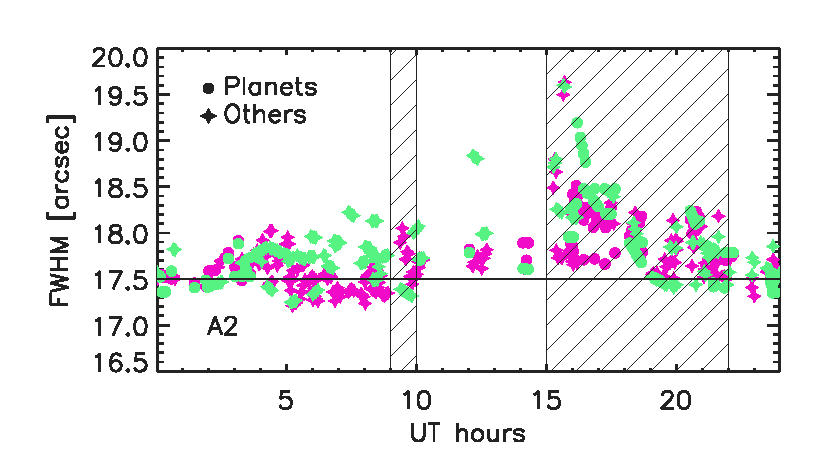
\includegraphics[clip=true, trim={0.5cm, 0.5cm, 0.5cm, 0.5cm}, width=0.4875\textwidth]{Figures/Beam_monitoring_with_otfs_vs_ut_compare_pointings_a2.pdf}
    \caption[Beam size monitoring comparison]{Beam size monitoring
      comparison. The FWHM estimates from a 2D Gaussian fit on the map
      of OTF scans toward bright sources ('OTF'-labeled pink data
      points) are compared to FWHM estimates that are obtained by
      interpolating the smoothed pointing-based FWHM at the time of
      the scans ('Pointing'-labeled light green data points).}
\label{fig:beam_monitoring_compare}
\end{center}
\end{figure}
%
Figure~\ref{fig:beam_monitoring_compare} shows two different FWHM
estimates for the same data set: the best-fitting FWHM estimates on
the map are compared with the interpolation from the pointing-based
FWHM monitoring. The two estimates are well in agreement with each
other, although the pointing-based estimates have more dispersion and
a few outliers.

%As a summary, we have evidenced a systematic beam size variation with
%the observation time using two different data sets: a series of OTF
%scans of bright sources and pointing scans. The beam size
%variation is i) reproducible from a campaign to another, stable
%with ii) the data set and iii) the sources. It consists of a beam
%broadening during afternoons and an increase of the dispersion during
%sunrises. \new{The \afternoon\ beam-size variation effect mainly
%originates from deformations of the $30\,\rm{m}$ primary mirror subject
%to the Sun irradiation, while anomalous refraction also play a
%role.}  
%The most impacted
%observing periods are well discarded using the baseline selection
%criteria discussed in Sect.~\ref{se:data_selection}.


%*************************************************************************
%
%   SEE CALIBRATION_2 FOR THE SECOND PART
%
%************************************************************************


%---------------------------------------------------------------------
%	BASELINE CALIBRATION
%---------------------------------------------------------------------
%\subsection{Baseline calibration}
%\label{se:baseline_calibration}



%---------------------------------------------------------------------
%	PHOTOMETRIC CORRECTION
%---------------------------------------------------------------------
%\subsection{Photometric correction}
%\label{se:photometric_correction}
